% !TeX spellcheck = cs_CZ
%{\tikzset{external/prefix={tikz/FYZII/}}
% \tikzset{external/figure name/.add={ch10_}{}}
%---------------------------------------------------------------------------------------------------
% file fey2ch10.tex
%---------------------------------------------------------------------------------------------------
%=========================== Kapitola: Dielektrika =================================================
\setchaptertoc
\chapter{Dielektrika}\label{fyz:IIchapX}
  \section{Permitivita}\label{fyz:IIchapXsecI}

    Na tomto místě začneme hovořit o další z charakteristických vlastností látky nacházející se pod
    vlivem elektrického pole. V jedné z předcházejících kapitol jsme se zabývali vlastnostmi
    \emph{vodičů}, v nichž se účinkem elektrického pole náboje volně přemisťují do takových míst, že
    uvnitř vodiče nezůstane žádné pole. Nyní budeme hovořit o \emph{izolantech}, tedy o látkách,
    které elektřinu nevedou. Na první pohled by se mohlo zdát, že se s nimi v elektrickém poli
    nestane vůbec nic. Ale Faraday pomocí jednoduchého elektroskopu a deskového kondenzátoru
    objevil, že tomu tak není. Jeho pokusy ukázaly, že kapacita takového kondenzátoru
    \emph{vzroste}, když se mezi jeho elektrody vloží izolant. Vyplní-li izolant prostor mezi
    elektrodami, kapacita se zvětší \(\varepsilon_r\)-krát, přičemž koeficient \(\varepsilon_r\)
    závisí pouze na vlastnostech izolační látky. Izolační látky se také nazývají \emph{dielektrika};
    součinitel \(\varepsilon_r\) je tedy vlastností dielektrika a nazývá se \emph{relativní
    permitivita}. Relativní permitivita vakua je, samozřejmě, rovna jedné.  

    Naší úlohou je nyní vysvětlit, proč vůbec nějaký elektrický efekt nastává, jsou-li izolanty
    opravdu izolanty a elektřinu nevedou. Vyjdeme z experimentálního faktu, že kapacita vzrůstá a
    pokusíme se vymyslet, co by se přitom mohlo dít. Uvažujme deskový kondenzátor s nějakými náboji
    na povrchu vodičů, řekněme se záporným nábojem na horní a s kladným nábojem na dolní elektrodě.
    Předpokládejme, že vzdálenost mezi elektrodami je \(d\) a plošný obsah každé elektrody je \(S\).
    Jak jsme viděli už dříve, kapacita kondenzátoru je
    \begin{equation}\label{fyz:eq907}
      C = \dfrac{\varepsilon_0S}{d}
    \end{equation}
    a náboj souvisí s napětím na kondenzátoru podle vztahu
    \begin{equation}\label{fyz:eq908}
      Q = CU.
    \end{equation}

    Experimentálním faktem je, že vložíme-li mezi desky kus izolantu, například skla nebo plexiskla,
    zjistíme, že se kapacita zvětší. To ovšem znamená, že při témže náboji se napětí snížilo. Ale
    napětí je integrálem elektrického pole počítaným napříč kondenzátorem; musíme tedy udělat závěr,
    že uvnitř kondenzátoru se zeslabilo elektrické pole, i když náboje na deskách zůstávají
    nezměněny.

    \begin{figure}[ht!] %\ref{fyz:fig705}
      \centering
      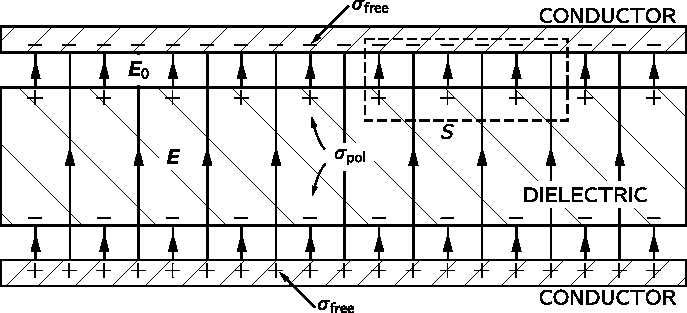
\includegraphics[width=0.9\linewidth]{fyz_fig705.pdf}
      \caption{Deskový kondenzátor s dielektrikem. Vyznačeny jsou siločáry elektrického pole \(E\).
               (\cite[s.~175]{Feynman02})}
      \label{fyz:fig705}
    \end{figure}

    Jak je to možné? Máme větu, pocházející od Gausse, která nám říká, že tok elektrického pole
    uzavřenou plochou je v přímém vztahu s náboji uvnitř plochy. Uvažujme gaussovskou plochu \(S\)
    vyznačenou na obr. \ref{fyz:fig705} čárkovaně. Protože elektrické pole se v přítomnosti
    dielektrika zeslabilo, usuzujeme, že celkový náboj uvnitř plochy musí být menší, než byl bez
    látky. Pak existuje jediný možný závěr a ten je, že na povrchu dielektrika musí sídlit kladné
    náboje. Protože se sice pole zeslabilo, ale ne na nulu, očekáváme, že tento kladný náboj je
    menší než záporný náboj na vodiči. Celý úkaz by bylo možné vysvětlit, kdybychom nějak uměli
    pochopit, proč se při umístění dielektrické látky do elektrického pole na jednom povrchu
    indukuje kladný a na druhém záporný náboj.

    Něco takového bychom očekávali v případě vodiče. Mějme například kondenzátor se vzdáleností
    \(d\) mezi elektrodami a vložme mezi ně neutrální vodič, jehož tloušťka je \(b\) (obr.
    \ref{fyz:fig706}). Elektrické pole indukuje kladný náboj na jeho horním povrchu a záporný náboj
    na jeho dolním povrchu, takže uvnitř vodiče pole není. Ve zbývajícím prostoru je pole totéž,
    jako by bylo bez vodiče, neboť je rovno plošné hustotě náboje dělené \(\varepsilon_0\) ale
    vzdálenost, přes kterou musíme integrovat, abychom dostali napětí (rozdíl potenciálů), se
    zmenšila.

    Napětí je
    \begin{equation*}
      U = \dfrac{U}{\varepsilon_0}(d-b).
    \end{equation*}
    Výsledný výraz pro kapacitu je stejný jako (\ref{fyz:eq907}), ale \(d\) je nahrazeno rozdílem
    \((d - b)\)
    \begin{equation}\label{fyz:eq909}
      C = \dfrac{\varepsilon_0S}{d\left[1 - (b/d)\right]}
    \end{equation}
    Kapacita se zvětšila v poměru, jenž závisí na \((b/d)\), tj. na poměrné části objemu, kterou
    zaujal vodič.

    \begin{figure}[ht!] %\ref{fyz:fig706}
      \centering
      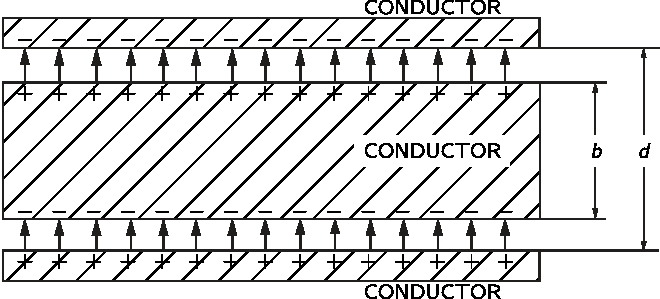
\includegraphics[width=0.9\linewidth]{fyz_fig706.pdf}
      \caption{Vložíme-li mezi elektrody deskového kondenzátoru vodivou desku, indukované náboje
               zeslabí pole uvnitř vodiče na nulovou hodnotu. (\cite[s.~175]{Feynman02})}
      \label{fyz:fig706}
    \end{figure}

    To nám však poskytuje zřejmý model toho, co se děje s dielektriky - uvnitř látky se nachází
    množství tenkých vodivých vrstev. S takovým modelem je však spojena jedna obtíž - má významnou
    osu, normálu k vrstvám, zatímco většina dielektrik takovou osu nemá. Ale tuto obtíž je možno
    vyloučit, uděláme-li předpoklad, že všechny izolační látky obsahují malé navzájem izolované
    vodivé koule, jak ukazuje obr. \ref{fyz:fig707}. Permitivita je vysvětlována působením nábojů,
    které by byly indukovány na každé kuličce. Je to jeden z prvních fyzikálních modelů dielektrika,
    použitých na vysvětlení jevu pozorovaného Faradayem. Konkrétněji řečeno, předpokládalo se, že
    každý z atomů látky je dokonalým vodičem, ale izolovaným od jiných atomů. Relativní permitivita
    \(\varepsilon_0\) bude záviset na tom, jakou část objemu zabírají vodivé koule. Dnes však tento
    model nepoužíváme.

    \begin{figure}[ht!] %\ref{fyz:fig707}
      \centering
      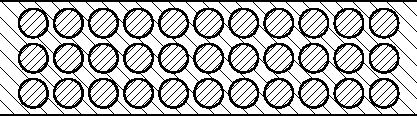
\includegraphics[width=0.9\linewidth]{fyz_fig707.pdf}
      \caption{Model dielektrika: malé vodivé kuličky zapuštěné do idealizovaného izolátoru
               (\cite[s.~176]{Feynman02})}
      \label{fyz:fig707}
    \end{figure}

  \section{Vektor elektrické polarizace P}\label{fyz:IIchapXsecII} 
    Pokračujeme-li v naší analýze, přijdeme na to, že představa o oblastech s dokonalou vodivostí a
    izolací mezi nimi není podstatná. Každá z malých kuliček se chová jako dipól, jehož moment je
    indukován vnějším polem. Jediná věc, jež je pro pochopení dielektrik podstatná je ta, že v
    dielektrické látce je indukováno mnoho malých dipólů. To, zda se dipóly indukují proto, že
    existují vodivé malé kuličky, nebo z nějakého jiného důvodu, je bezvýznamné.

    Proč by pole mělo v atomu indukovat dipólový moment, není-li atom vodivou koulí? O této otázce
    budeme mluvit mnohem podrobněji v následující kapitole, která bude věnována vnitřním procesům v
    dielektrických látkách. Zde však uvedeme jeden příklad, abychom ilustrovali možný mechanizmus.
    Kladný náboj atomu je v jádře, jež je obklopeno zápornými elektrony. Orbity nebo vlnové balíky
    elektronů (nebo jakékoliv zobrazení použité v kvantové mechanice) jsou v nějaké míře pokřiveny
    (obr. \ref{fyz:fig708}); těžiště záporného náboje se posune a nebude už splývat s kladným
    nábojem jádra. My jsme už o takovém rozdělení náboje hovořili. Díváme-li se na něj z velké
    vzdálenosti, je taková neutrální konfigurace v prvním přiblížení ekvivalentní malému dipólu.

    \begin{figure}[ht!]
      \centering
      \subcaptionbox{\label{fyz:fig708a}}{\luafigure[0.45]{fyz_fig708a.pdf}}
      \subcaptionbox{\label{fyz:fig708b}}{\luafigure[0.45]{fyz_fig708b.pdf}}
      \label{fyz:fig708}
      \caption{Rozdělení elektronů v atomu nacházejícím se v elektrickém poli se vzhledem k jádru
              posune. (\cite[s.~177]{Feynman02})}
    \end{figure}

    Asi je rozumné předpokládat, že není-li pole příliš silné, velikost indukovaného dipólového
    momentu bude přímo úměrná poli. Slabé pole tedy posune náboje jen o malý kousíček, zatímco silné
    pole je posune víc, a to přímo úměrně poli, jen když posunutí nebude příliš velké. Do konce této
    kapitoly budeme dipólový moment považovat za přesně přímo úměrný poli.

    Dále budeme předpokládat, že v každém atomu jsou náboje \(q\) ve vzájemné vzdálenosti
    \(\vec{δ}\) takže \(q\vec{δ}\) je elektrický dipólový moment připadající na jeden atom.
    (\(\vec{δ}\) používáme proto, neboť \(d\) jsme už použili pro vzdálenost elektrod.) Je-li v
    jednotkovém objemu \(N\) atomů, bude \textbf{dipólový moment jednotkového objemu} roven
    \(Nq\vec{δ}\). Tento elektrický dipólový moment připadající na jednotkový objem budeme označovat
    vektorem \(\vec{P}\). Není třeba zdůrazňovat, že leží ve směru jednotlivých dipólových momentů,
    tj. ve směru posunutí nábojů \(\vec{δ}\).
    \begin{equation}\label{fyz:eq910}
      \vec{P} = Nq\vec{δ}
    \end{equation}

    Obecně se bude \(\vec{P}\) v dielektriku měnit od místa k místu. Ale v každém bodě látky je
    přímo úměrné elektrickému poli. Součinitel této úměrnosti je určen tím, jak snadno se elektron
    posune, a závisí na druhu atomů v látce.
    
    O tom, co doopravdy určuje, jak se tento součinitel chová, jak přesně konstantní je ve velmi
    silných polích a co se děje uvnitř různých látek, budeme mluvit později. V této chvíli budeme
    prostě předpokládat, že existuje mechanizmus, jímž se indukuje elektrický dipólový moment přímo
    úměrný elektrickému poli.

  \section{Polarizační náboje}\label{fyz:IIchapXsecIII}   
    Nyní prozkoumejme, co z tohoto modelu vyplývá pro teorii kondenzátoru vyplněného dielektrikem.
    Nejdříve uvažujeme destičku z látky, která má určitý elektrický dipólový moment připadající na
    jednotkový objem. Vznikne v důsledku toho v průměru nějaká hustota náboje v látce? Ne, je-li
    \(\vec{P}\) homogenní. Mají-li kladné a záporné náboje po posunutí stejné hustoty náboje, z
    jejich posunutí nevzniká v objemu žádný výsledný náboj. Na druhé straně, kdyby \(\vec{P}\) bylo
    v jednom místě větší a v druhém místě menší, znamenalo by to, že se do některé oblasti přesunulo
    více náboje, než se z ní vysunulo ven; tehdy bychom mohli očekávat nenulovou objemovou hustotu
    náboje. V případě deskového kondenzátoru předpokládáme, že \(\vec{P}\) je homogenní, takže je
    nutné prozkoumat pouze to, co se děje na povrchu. Na jednom povrchu se záporné náboje -
    elektrony efektivně vysunuly do vzdálenosti \(δ\), zatímco na druhém povrchu se posunuly dovnitř
    a zanechaly určitý kladný náboj na vzdálenosti \(δ\). Jak ukazuje obr. \ref{fyz:fig709}, na
    povrchu vznikne plošná hustota náboje, který budeme nazývat \textbf{povrchovým polarizačním
    nábojem}.

    Tento náboj je možné vypočítat následujícím způsobem. Počet elektronů, které se objeví na
    povrchu destičky je roven součinu jejího plošného obsahu \(S\), počtu elektronů v jednotkovém
    objemu \(N\) a posunutí \(δ\), o němž zde předpokládáme, že nastane kolmo k povrchu. Výsledný
    náboj dostaneme vynásobením této hodnoty nábojem elektronu \(q_e\). Abychom dostali plošnou
    hustotu polarizačního náboje indukovaného na povrchu, musíme výsledek dělit plošným obsahem
    \(S\). Velikost plošné hustoty náboje tedy bude
    \begin{equation*}
      σ_{\text{pol}}=Nq_eδ.
    \end{equation*}
    To je však právě rovno velikosti \(P\) vektoru elektrické polarizace \(\vec{P}\), daného vztahem
    (\ref{fyz:eq910}), tj. 
    \begin{equation}\label{fyz:eq911}
      σ_{\text{pol}} = P.
    \end{equation}
    \emph{Plošná hustota náboje na povrchu látky je rovna elektrické polarizaci v jejím vnitřku.}
    Povrchový náboj je samozřejmě kladný na jedné straně a záporný na opačné straně povrchu.

    \begin{figure}[ht!] %\ref{fyz:fig709}
      \centering
      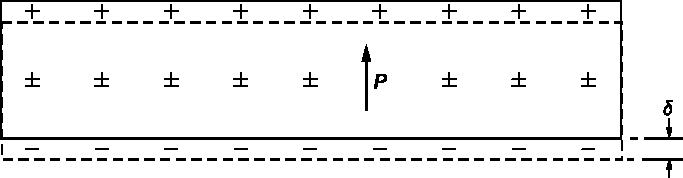
\includegraphics[width=1\linewidth]{fyz_fig709.pdf}
      \caption{Dielektrická vrstva v homogenním poli. Kladné náboje jsou posunuty do vzdálenosti
              \(δ\) vzhledem k záporným. (\cite[s.~177]{Feynman02})}
      \label{fyz:fig709}
    \end{figure}
    
    Dále předpokládejme, že naše deska představuje dielektrikum v rovinném kondenzátoru. Na
    \emph{elektrodách} kondenzátoru se také nachází plošný náboj, jehož hustotu označíme
    \(σ_{\text{free}}\), neboť ve vodiči se náboje mohou „volně“ pohybovat. Jde, samozřejmě, o
    náboj, který jsme dodali při nabíjení kondenzátoru. Je nutné zdůraznit, že \(σ_{\text{pol}}\)
    existuje jen proto, že existuje \(σ_{\text{free}}\). Odstraní-li se vybitím kondenzátoru
    \(σ_{\text{free}}\), vymizí také \(σ_{\text{pol}}\). Neodejde však vodičem, kterým se vybije
    kondenzátor, ale pohybem zpět dovnitř látky, a to rozptýlením polarizace uvnitř látky.

    Nyní můžeme na gaussovskou plochu \(S\), znázorněnou na obr. \ref{fyz:fig705}, použít Gaussův
    zákon. Elektrické pole \(\vec{E}\) v dielektriku je rovno celkové plošné hustotě náboje dělené
    \(ϵ_0\). Je zřejmé, že \(σ_{\text{pol}}\) a \(σ_{\text{free}}\) mají opačná znaménka, takže
    \begin{equation}\label{fyz:eq912}
      E = \dfrac{σ_{\text{free}} - σ_{\text{pol}}}{\varepsilon_0}.
    \end{equation}

    Všimněme si, že pole \(E_0\) mezi kovovou elektrodou a povrchem dielektrika je větší než pole
    \(E\); odpovídá pouze hustotě \(σ_{\text{free}}\). Zde se však zajímáme o pole uvnitř
    dielektrika. Vyplňuje-li dielektrikum téměř celou mezeru mezi elektrodami, je toto pole
    rozprostřeno prakticky v celém objemu uvnitř kondenzátoru. Použijeme-li vztah (\ref{fyz:eq911}),
    můžeme napsat
    \begin{equation}\label{fyz:eq913}
      E = \dfrac{σ_{\text{free}} - P}{\varepsilon_0}.
    \end{equation}
    Z této rovnice se nemůžeme dovědět, jaké je elektrické pole, bez znalosti \(P\). Zde však
    předpokládáme, že \(P\) závisí na \(E\), konkrétně, že je přímo úměrné \(E\). Tato přímá
    úměrnost se obvykle zapisuje takto:
    \begin{equation}\label{fyz:eq914}
      \vec{P}=χϵ_0\vec{E}.
    \end{equation}
    Konstanta \(χ\) (řecké „chí“) se nazývá \textbf{elektrická susceptibilita dielektrika}.

    Potom vztah (\ref{fyz:eq913}) nabude tvaru
    \begin{equation}\label{fyz:eq915}
      E=\dfrac{σ_{\text{free}}}{ϵ_0}\dfrac{1}{(1+χ)},
    \end{equation}
    podle kterého se pole zmenšilo v poměru \(1/(1+χ)\).

    Napětí mezi elektrodami vyjadřuje integrál elektrického pole. Protože jde o homogenní pole,
    integrál je redukován na součin intenzity pole \(E\) a vzdálenosti \(d\) mezi elektrodami.
    Dostáváme
    \begin{equation}
      U = Ed = \dfrac{σ_{\text{free}}dϵ0(1+χ)
    \end{equation}

    \begin{figure}[ht!] %\ref{fyz:fig710}
      \centering
      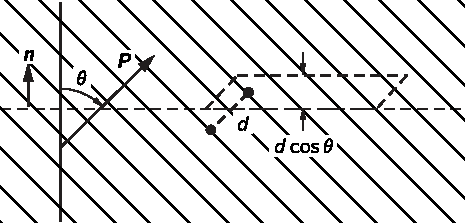
\includegraphics[width=0.9\linewidth]{fyz_fig710.pdf}
      \caption{Náboj, který prošel v dielektriku elementární myšlenou ploškou, je přímo úměrný
               složce vektoru \(\vec{P}\) ve směru normály k ploše. (\cite[s.~179]{Feynman02})}
      \label{fyz:fig710}
    \end{figure}

    \begin{figure}[ht!] %\ref{fyz:fig711}
      \centering
      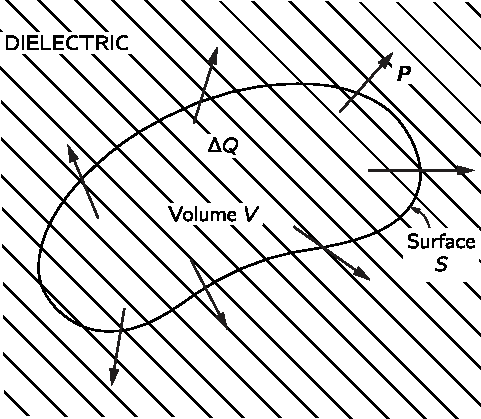
\includegraphics[width=0.9\linewidth]{fyz_fig711.pdf}
      \caption{Nehomogenní polarizace \(\vec{P}\) může vést ke vzniku náboje v objemu dielektrika.
               (\cite[s.~707]{Feynman02})}
      \label{fyz:fig711}
    \end{figure}

  \section{Elektrostatické rovnice pro dielektrika}\label{fyz:IIchapXsecIV}
  
  \section{Pole a síly v přítomnosti dielektrik}\label{fyz:IIchapXsecV}

    \begin{figure}[ht!] %\ref{fyz:fig712}
      \centering
      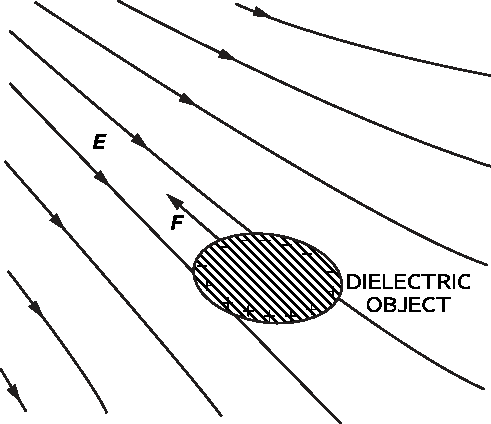
\includegraphics[width=0.5\linewidth]{fyz_fig712.pdf}
      \caption{V nehomogenním poli působí na dielektrické těleso síla směřující do prostoru s vyšší
              intenzitou pole. (\cite[s.~184]{Feynman02})}
      \label{fyz:fig712}
    \end{figure}

    \begin{figure}[ht!] %\ref{fyz:fig713}
      \centering
      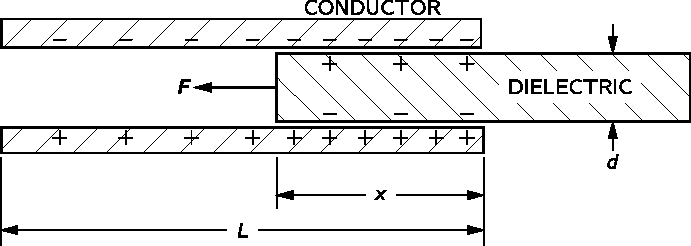
\includegraphics[width=0.5\linewidth]{fyz_fig713.pdf}
      \caption{Sílu působící v deskovém kondenzátoru na dielektrickou destičku můžeme vypočítat
               použitím principu zachování energie. (\cite[s.~707]{Feynman02})}
      \label{fyz:fig713}
    \end{figure}

  \section{Příklady a cvičení}\label{fyz:IIchapXsecVI}



\todo[inline]{Kapitola fey2ch10 je nedodělaná, obsahuje pouze obrázky}
%} %tikzset
%---------------------------------------------------------------------------------------------------
